\documentclass[tikz,border=10pt]{standalone}
\usepackage[T1]{fontenc}
\usepackage{mathpazo}
\usepackage{amsmath,amssymb}
\usetikzlibrary{arrows.meta, positioning, calc, fit}

\definecolor{stblue}{HTML}{7B97AD}
\definecolor{rwgold}{HTML}{B8995E}
\definecolor{sage}{HTML}{7A9A7E}
\definecolor{dkbrown}{HTML}{3D3530}
\definecolor{wmgray}{HTML}{7B7067}
\definecolor{cream}{HTML}{F9F6F0}
\definecolor{border}{HTML}{D4C9B8}
\definecolor{terracotta}{HTML}{C47A6A}

\begin{document}
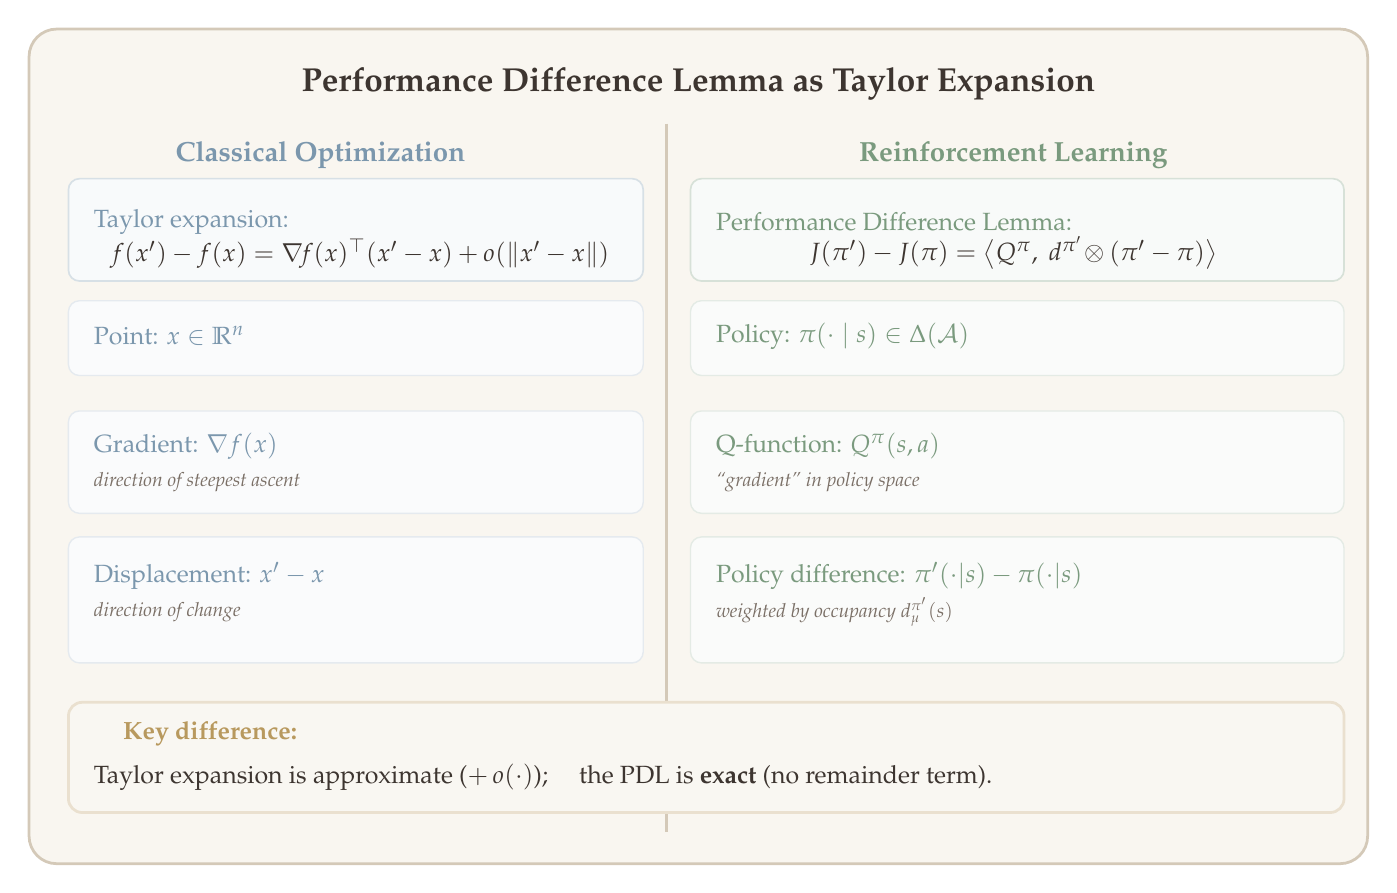
\begin{tikzpicture}[
  >={Stealth[length=2.5mm, width=2mm]},
  hdr/.style={font=\normalsize\bfseries, text=dkbrown},
  row/.style={font=\small, text=dkbrown, anchor=west, align=left},
  mth/.style={font=\small, text=#1, anchor=west},
]

% Background
\fill[cream, rounded corners=10pt] (-0.5,-6.8) rectangle (16.5,3.8);
\draw[border, rounded corners=10pt, line width=1pt] (-0.5,-6.8) rectangle (16.5,3.8);

% Title
\node[font=\large\bfseries, text=dkbrown] at (8.0,3.1)
  {Performance Difference Lemma as Taylor Expansion};

% === Column headers ===
\node[hdr, text=stblue] at (3.2,2.2) {Classical Optimization};
\node[hdr, text=sage] at (12.0,2.2) {Reinforcement Learning};

% Divider
\draw[border, line width=1pt] (7.6,2.6) -- (7.6,-6.4);

% === Row labels (left column) ===
\def\rA{1.2}
\def\rB{-0.2}
\def\rC{-1.8}
\def\rD{-3.6}
\def\rE{-5.6}

% Row 1: Taylor expansion / PDL
\draw[stblue!30, line width=0.6pt, rounded corners=4pt, fill=stblue!5]
  (0.0,\rA+0.7) rectangle (7.3,\rA-0.6);
\draw[sage!30, line width=0.6pt, rounded corners=4pt, fill=sage!5]
  (7.9,\rA+0.7) rectangle (16.2,\rA-0.6);

\node[font=\footnotesize\bfseries, text=wmgray] at (-0.0,\rA+0.5) {};
\node[mth=stblue] at (0.2,\rA+0.15) {Taylor expansion:};
\node[font=\small, text=dkbrown] at (3.7,\rA-0.25) {$f(x') - f(x) = \nabla\! f(x)^\top(x' - x) + o(\|x'-x\|)$};
\node[mth=sage] at (8.1,\rA+0.15) {Performance Difference Lemma:};
\node[font=\small, text=dkbrown] at (12.0,\rA-0.25) {$J(\pi') - J(\pi) = \bigl\langle Q^\pi,\; d^{\pi'}\!\otimes(\pi' - \pi)\bigr\rangle$};

% Row 2: Point / Policy
\draw[stblue!20, line width=0.5pt, rounded corners=4pt, fill=stblue!4]
  (0.0,\rB+0.55) rectangle (7.3,\rB-0.4);
\draw[sage!20, line width=0.5pt, rounded corners=4pt, fill=sage!4]
  (7.9,\rB+0.55) rectangle (16.2,\rB-0.4);

\node[mth=stblue] at (0.2,\rB+0.1) {Point: $x \in \mathbb{R}^n$};
\node[mth=sage] at (8.1,\rB+0.1) {Policy: $\pi(\cdot \mid s) \in \Delta(\mathcal{A})$};

% Row 3: Gradient / Q-function
\draw[stblue!20, line width=0.5pt, rounded corners=4pt, fill=stblue!4]
  (0.0,\rC+0.75) rectangle (7.3,\rC-0.55);
\draw[sage!20, line width=0.5pt, rounded corners=4pt, fill=sage!4]
  (7.9,\rC+0.75) rectangle (16.2,\rC-0.55);

\node[mth=stblue] at (0.2,\rC+0.3) {Gradient: $\nabla f(x)$};
\node[font=\scriptsize\itshape, text=wmgray, anchor=west] at (0.2,\rC-0.15) {direction of steepest ascent};
\node[mth=sage] at (8.1,\rC+0.3) {Q-function: $Q^\pi(s,a)$};
\node[font=\scriptsize\itshape, text=wmgray, anchor=west] at (8.1,\rC-0.15) {``gradient'' in policy space};

% Row 4: Displacement / Policy difference
\draw[stblue!20, line width=0.5pt, rounded corners=4pt, fill=stblue!4]
  (0.0,\rD+0.95) rectangle (7.3,\rD-0.65);
\draw[sage!20, line width=0.5pt, rounded corners=4pt, fill=sage!4]
  (7.9,\rD+0.95) rectangle (16.2,\rD-0.65);

\node[mth=stblue] at (0.2,\rD+0.45) {Displacement: $x' - x$};
\node[font=\scriptsize\itshape, text=wmgray, anchor=west] at (0.2,\rD) {direction of change};
\node[mth=sage] at (8.1,\rD+0.45) {Policy difference: $\pi'(\cdot|s) - \pi(\cdot|s)$};
\node[font=\scriptsize\itshape, text=wmgray, anchor=west] at (8.1,\rD) {weighted by occupancy $d^{\pi'}_\mu(s)$};

% Row 5: Key difference
\draw[rwgold!30, line width=1pt, rounded corners=5pt, fill=rwgold!8]
  (0.0,\rE+0.85) rectangle (16.2,\rE-0.55);

\node[font=\small\bfseries, text=rwgold] at (1.8,\rE+0.45)
  {Key difference:};
\node[font=\small, text=dkbrown, anchor=west, align=left] at (0.2,\rE-0.1)
  {Taylor expansion is approximate ($+\, o(\cdot)$); \quad the PDL is \textbf{exact} (no remainder term).};

\end{tikzpicture}
\end{document}
